\chapter{Evaluation and Findings}
    This chapter focuses on the interpretation of performance metrics and typical error patterns by analysing typical error patterns in the test sets and conducting exploratory tests to validate initial assumptions.

\section{Model Performance}
    The model’s overall accuracy on the held-out test set is 0.966, with matching macro F1 and weighted average. This shows it performs evenly across both classes. Precision and recall reveal biased cases are detected very well (recall 0.993) with some false alarms (precision 0.937), meaning a small portion of neutral cases are incorrectly labeled as biased. The confusion matrix confirms this with 10 false positives and only 1 false negative in 325 examples. The false positive rate is 0.057 and the false negative rate is 0.007. Overall, this suggests the model favors detecting bias at the risk of some over-flagging, which fits typical needs for bias detection where missing bias is costlier than false alarms.

        \vspace{0.8em}
        \begin{table}[H]
            \centering
            \begin{tabular}{lccc}
            \toprule
            \textbf{Class} & \textbf{Precision} & \textbf{Recall} & \textbf{F1 Score} \\
            \midrule
            Neutral (0) & 0.994 & 0.943 & 0.968 \\
            Biased (1)  & 0.937 & 0.993 & 0.964 \\
            \bottomrule
            \end{tabular}
            \caption{Per-class precision, recall, and F1 score on the test set}
        \end{table}

        \vspace{0.8em}
        \begin{table}[H]
            \centering
            \begin{tabular}{lc}
            \toprule
            \textbf{Metric} & \textbf{Value} \\
            \midrule
            Accuracy & 0.966 \\
            Macro-average F1 Score & 0.966 \\
            Weighted-average F1 Score & 0.966 \\
            False Positive Rate & 0.057 \\
            False Negative Rate & 0.007 \\
            \bottomrule
            \end{tabular}
            \caption{Overall evaluation metrics on the test set}
        \end{table}

        \begin{figure}[ht]
            \centering
            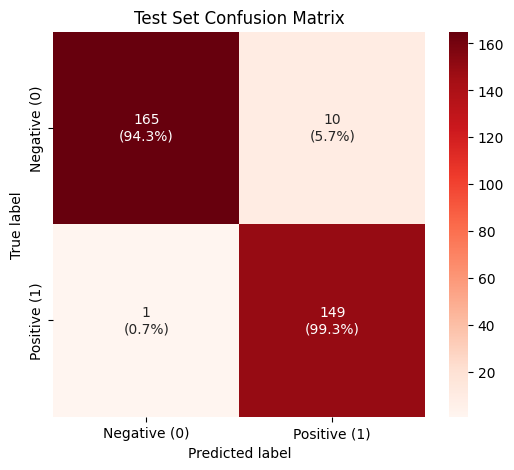
\includegraphics[width=0.75\textwidth]{test_set_confusion_matrix.png}
            \caption[Confusion matrix on the test dataset]{Confusion matrix of the model on the test dataset, showing true vs. predicted labels with counts}
            \label{fig:test_confusion_matrix}
        \end{figure}

    False positives and false negatives make up only a small share of the total predictions, but they point to recurring patterns in the model’s errors. These cases were grouped by shared features to enable a structured analysis of likely causes.\footnote{Refer to the appendix for all misclassified examples, including English source texts and German translations.}

    \paragraph{State and Governance Entity Terms}

    Sentences containing political, legal, or governance-related terminology were misclassified the most (6/10 cases). Terms such as president, police officers, heads of state and government, and political leaders were flagged as biased, despite the absence of gendered language in the German translation. The model may struggle to distinguish between genuinely biased constructions and content related to institutional or geopolitical domains. Another possible explanation is the strong male association of such terms in real-world data, which may influence model behavior through learned co-occurrence patterns \parencite{kroeberItsLongWay2022}.

    \paragraph{Training Dataset Error Causing a False Positive}

    One false positive appears to stem from an inconsistency within the training dataset. The English sentence "[...] or would you go to a surgeon?" was translated as "[...] oder von einem Menschen, der als Chirurg ausgebildet wurde [...]?". This example originates from the mGeNTE dataset and is labeled as unbiased. The German translation attempts to avoid using "der Chirurg" (m.) by phrasing it as "a person trained as a surgeon," presumably to circumvent the generic masculine. However, the word "Chirurg" still appears in the translation in its masculine form. The model correctly identified this gendered term and flagged it, despite the label indicating neutrality. From a bilingual perspective, the model’s detection is a true positive and the false flagging points to a labeling inconsistency in the dataset.

    \paragraph{Religious identities}
    
    One false negative involved a sentence concerning the immigration of muslims. "Muslims" was translated using the generic masculine form "Muslime", yet the model failed to recognize this instance as biased. Since the sentence does not provide a clear reason for why it was misclassified, this issue will be further analysed using exploratory testing (\autoref{section:exploratory_testing}).

    \paragraph{Issues with GFL and Semantically Gendered Terms}

    Two instances were incorrectly flagged as biased due to the use of GFL. The gender-ambiguous terms "specialists" and "recipient" were translated as "Sachkundigen" and "Rezipierende," respectively, both using neutral rewording. The false detection here reflects insufficient understanding of GFL forms.

    Additionally, one semantically gendered term, "uncle," translated as "Onkel," was flagged, pointing towards difficulty in distinguishing inherently gendered terms from translation-induced gender bias. This assumption will be tested for consistency in \autoref{subsection:generalization_performance_on_unseen}.

\section{Generalization performance on unseen data} \label{subsection:generalization_performance_on_unseen}
    To assess how well these findings generalize, the results from the handcrafted test set are now analysed. As explained in \autoref{subsection:eval_dataset}, the handcrafted test set was curated to expose potential failure modes and edge cases that may not be captured by standard evaluation.\footnote{Refer to the appendix for the handcrafted test results and confidence scores.}

    \subsection{Weaknesses}
    \autoref{tab:false_positives_with_conf} shows all of its false predictions. Consistent with the results from the held-out test set, these errors involve semantic gender distinctions and GFL variants. It is important to note that the test set did include more semantic gender examples, such as “sister,” “boy,” and “father” in ambiguous contexts, which the model did not flag. Sentence 5 with “mother” was flagged, but with low confidence. It can be concluded that this limitation stems from insufficient training data for semantically gendered words. The model recognizes a pattern but lacks enough instances to confidently classify. The remaining three cases share the same sentence structure but use different GFL forms. The model flagged some sentences using the pair form and gender-inclusive characters (the colon) as biased, with over 95\% confidence. It did however correctly identify the user of the gender star and neutral rewording of "teacher" to "Lehrende" as unbiased, also with a confidence of over 95\%.
    
    This reflects the known limitation of the dataset, where the limited availability of high-quality natural GFL data required supplementing it with lower-quality synthetic examples. Still, the correct classification in some cases suggests that the model may be capable of handling GFL more reliably if more representative data were available.

    \vspace{0.8em}
        \begin{table}[ht]
        \centering
        \begin{tabular}{|c|p{5cm}|p{5cm}|c|c|}
        \hline
        \textbf{Index} & \textbf{English} & \textbf{German} & \makecell[c]{Neutral \\ Prob \%} & \makecell[c]{Biased \\ Prob \%} \\
        \hline
        5 & My mother is an engineer. & Meine Mutter ist Ingenieurin. & 44.1 & 55.9 \\
        16 & Engineers are kind and hard-working & Ingenieure und Ingenieurinnen sind lieb und fleißig & 0.08 & 99.92 \\
        18 & Teachers are kind and hard-working & Lehrer:innen sind lieb und fleißig & 3.1 & 96.9 \\
        19 & Teachers are kind and hard-working & Lehrerinnen und Lehrer sind lieb und fleißig & 0.05 & 99.95 \\
        \hline
        \end{tabular}
        \caption{Handcrafted test sentences with incorrect model predictions and confidence scores (percent)}
        \label{tab:false_positives_with_conf}
        \end{table}

\subsection{Strengths}
The performance metrics earlier already imply that the model performs strongly in detecting genuinely biased cases. This is supported by the handcrafted test set: no clearly biased sentence was missed, and out of these, not a single one received a confidence score below 90\%. The model also demonstrates the ability to distinguish between clearly gendered and neutral content. Generic sentences such as “How are you?”, translated as “Wie geht es dir?”, were correctly classified as neutral. Likewise, sentences taken from real job postings were consistently identified with high confidence (e.g., “The ideal candidate” → “Der ideale Kandidat” (m.) = biased). In total, all tested job posting examples reached confidence scores above 99\%. This indicates that the model is well-suited for handling practical use cases, which supports its applicability in real-world scenarios.

\section{Exploratory Testing} \label{section:exploratory_testing}
    To further investigate the unresolved misclassification of the religious identity sentence, the demo was used to test additional cases. The term "Muslims" was replaced with other religious terms, followed by "soldiers" to represent a non-religious but contextually relevant group, and concluded with "doctors," a typical example of a generic masculine translation.

    \vspace{0.8em}
    Sentence Under Investigation:
    \begin{quote}
    \textbf{English:} Here too the local people are frustrated by the immigration of Muslims and the hard line taken by the military.

    \textbf{German:} Hier wird die lokale Bevölkerung ebenfalls durch die Zuwanderung von Muslimen und das unnachsichtige Auftreten des Militärs schwer gebeutelt.
    \end{quote}

        \vspace{0.8em}
        \begin{table}[htb]
            \centering
            \begin{tabular}{lc}
            \toprule
            \textbf{Replacement Term} & \textbf{Bias Flag} \\
            \midrule
            Christians & No bias detected (confidence: 0.89) \\
            Jews & No bias detected (confidence: 0.93) \\
            Soldiers & No bias detected (confidence: 0.79) \\
            Doctors & No bias detected (confidence: 0.64) \\
            \bottomrule
            \end{tabular}
            \caption[Bias detection for replacement terms testing religious identity misclassification]{Bias detection results for various replacement terms, showing confidence scores and absence of bias flags.}
        \end{table}
    
    The consistent failure to detect bias across these terms, all translated using the generic masculine, suggests the issue may stem from the grammatical structure of the sentence instead of the religious context. 

    Testing formal features like punctuation and casing showed a clearer impact on the confidence. Removing the period dropped confidence to 0.84. Lowercasing "Muslims" lowered it to 0.83. Doing both together caused the confidence to fall to 0.58. Because the model is based on cased BERT, it relies on correct punctuation and capitalization for context. The limited training data increases the model’s sensitivity to such formal changes, causing performance to vary when cues like casing and punctuation are missing or altered. To confirm this effect, the insertion tests were repeated with both punctuation and casing removed. In these modified cases, "christians" was flagged as biased (confidence: 0.98), "soldiers" was not flagged (confidence: 0.63), and "doctors" was again flagged (confidence: 0.76).

    \vspace{0.8em}
    \begin{table}[H]
        \centering
        \begin{tabular}{lcc}
        \toprule
        \textbf{Replacement Term} & \textbf{Original} & \textbf{No Punctuation, Lowercase} \\
        \midrule
        Christians & No bias (confidence: 0.89) & Bias (confidence: 0.98) \\
        Jews & No bias (confidence: 0.93) & No bias (confidence: 0.51) \\
        Soldiers & No bias (confidence: 0.79) & No bias (confidence: 0.63) \\
        Doctors & No bias (confidence: 0.64) & Bias (confidence: 0.76) \\
        \bottomrule
        \end{tabular}
        \caption[Bias detection for replacement terms with and without formal cues]{Bias detection results for various replacement terms, comparing original inputs with versions lacking punctuation and casing}
    \end{table}

    One final hypothesis was that the term "local people" may influence the classification. In the original translation, it was rendered as "lokale Bevölkerung"; a neutral term that may give the impression of a gender-neutral subject. This could have caused the model to focus less on the gendered translation of "Muslims". To explore this, the term "local" was removed from the original sentence, changing the translation to "Auch hier sind die Menschen durch die Einwanderung von Muslimen und die harte Linie des Militärs frustriert."\footnote{This translation slightly differs in wording because it was generated using OpusMT. The version in the test set was likely manually translated by the mGeNTE creators.} The model correctly flagged this version as biased (confidence: 0.97). The presence of both a neutral and a gendered subject within the same sentence should be considered a factor that may reduce the model’s classification accuracy. At the same time, testing edge cases is inherently challenging due to the interaction of multiple subtle influences. While stepwise sentence modifications can help identify possible sources of misclassification, definitive conclusions remain difficult to establish.

    In this chapter, the model was evaluated in view of the research question. Its performance was analyzed on both a held-out dataset and a handcrafted dataset of unseen examples. Real-world texts, such as job postings, were used to test how the model performs in practice. Common error patterns were identified and grouped to better understand factors that influence misclassification, providing a basis for the conclusions in the next chapter.


 